\chapter{Notes \\
\small{\textit{-- Emmanuel Okoro and Spurthi Setty}}
\index{Notes} 
\index{Chapter!Notes}
\label{Chapter::Notes}}

\section{Project Mission Statement}
Empowering individuals to take control of their financial future by harnessing AI-driven analytics for intelligent budgeting, planning, and wealth creation.

\section{Key Stakeholders}
\subsection{Customers}
We have divided the customers into different user classes based on their intended frequency of using the application. We expect the Favored User Class to be those who use the application the most, and therefore a majority of the features will be catered for these groups. Disfavored users still interact directly with the system, however the scope of the project limits developing features that would be comprehensive enough for them. 

\subsubsection{Favored User Classes}
Since this application is a "Personal" finance tracker, the needs of individuals are prioritized, and we considered them as part of the favored user class as they derive direct value from the system. 

\begin{itemize}
    \item Working Individuals: This user group typically has to deal with rec curing bills pertaining to the cost of living (e.g., Rent, utilities, groceries, etc.), saving goals and unexpected expenses. They are favored since it is the largest target market which diverse financial needs which the application addresses. Features such as insights and recommendations, tax filing, and bank account integration can significantly assist these individuals with their financial management in the short and long term. 
    
    \item Students: Students often have a more limited income, if any, compared to working individuals. Their main concern is managing day-to-day expenses while staying within their financial means. They would benefit significantly from features like budgeting tools and insights and recommendations to budget their finances more efficiently. 
\end{itemize}
\subsubsection{Disfavored User Classes}
Disfavored user classes are those whose needs are not prioritized due to misalignment with the system’s goals, complexity, or high cost of implementation relative to benefit. While these user groups can derive some benefit from this application, it is not to the extent of the favored user classes. 

\begin{itemize}
    \item Small Business Owners: Small business owners often require tools for managing both personal and business finances. They may expect features like payroll management, invoicing, and business expense reporting. Their needs extend beyond personal finance tracking and may overlap with enterprise financial tools (e.g., QuickBooks). Supporting business-specific features would increase system complexity and development cost.
    
    \item Retail Investors: Retail investors often look for advanced financial tools to manage stocks, bonds, or other investments. They may expect integration with trading platforms or investment dashboards. Their needs are outside the scope of basic personal finance management and would require complex integrations with investment tools. Supporting this class would divert resources from core features like budgeting and spending insights.

\end{itemize}
\subsection{Oversight Stakeholders}
Oversight stakeholders ensure the system adheres to laws, regulations, and standards. They shape security, privacy, and regulatory compliance requirements.
\subsubsection{Regulatory Agencies}
\begin{itemize}
    \item Tax Authorities: This ensures compliance with tax laws, forms, and filing processes. They influence the requirements by making sure that the system supports automated tax calculations that align with the latest tax laws and is compatible with tax submission protocols (e.g., e-filing formats).
    
    \item Data Protection Agencies: This category of stakeholders includes agencies such as GDPR, CCPA, or HIPAA (if health-related financial data is handled) which enforce data privacy laws to protect users' personal and financial information. Thes stakeholders will largeley impact system and security requirements like end-to-end encryption for sensitive user data and data management options (e.g., opt-in/opt-out for data sharing, user data deletion on request).
    
    \item Consumer Protection Agencies: These stakeholders are responsible for safeguarding user rights and ensure transparency in the app’s financial recommendations. They ensure the app provides reliable and unbiased financial advice without promoting harmful spending habits.
\end{itemize}

\subsection{Supporting Stakeholders}
Supporting stakeholders provide resources, infrastructure, or services. They influence system integration and technical requirements to ensure the system functions as intended.

\subsubsection{API Providers}
\begin{itemize}
    \item Bank API Providers: Influence secure bank transaction integration and data retrieval performance. This is key for the Bank Account integration feature, and these stakeholders will have an impact on many of the quality requirements and technical specifications related to this feature.

    \item OCR API Providers: These providers drive requirements for accurate, automated receipt scanning (e.g., Google Vision, Amazon Textract). 
\end{itemize}

\subsubsection{Project Team}
\begin{itemize}
    \item Development Team: This group is responsible for implementing functional requirements and ensuring technical feasibility. They enable the app's core features, such as budgeting tools, insights generation, and tax filing capabilities. 
    
    \item System Administrators: This group manages the infrastructure, scalability, and up-time of the app and supports requirements related to system performance, monitoring, and security.

    \item Support Team: Provide ongoing assistance to users and ensure smooth operations post-launch. Influence requirements for logging, troubleshooting tools, and in-app user support features.

\end{itemize}

\subsection{Potential Conflicts among Stakeholders}

\subsubsection{Core Stakeholders vs. Supporting Stakeholders}
\textbf{Conflict:} Working Individuals and Students (Core Stakeholders) demand real-time data retrieval for features such as bank integration, insights, and receipt scanning. However, API Providers (Supporting Stakeholders), particularly Bank API Providers, may impose \textit{rate limits} on transaction data retrieval, which could affect system performance.

\textbf{Impact:} Delays in syncing data may frustrate users who expect instantaneous updates.

\textbf{Proposed Resolution:}
\begin{itemize}
    \item Implement data caching mechanisms to reduce the frequency of API calls.
    \item Negotiate premium access with API providers to increase rate limits.
    \item Clearly communicate data sync schedules to manage user expectations.
\end{itemize}

\subsubsection{Core Stakeholders vs. Regulatory Agencies}
\textbf{Conflict:} Data Protection Agencies (Regulatory Agencies) enforce strict privacy laws (e.g., GDPR, CCPA), which require explicit user consent for data collection and sharing. Core Stakeholders expect seamless, automated features (e.g., receipt scanning and bank integration) with minimal manual intervention.

\textbf{Impact:} Frequent consent pop-ups or manual approvals can disrupt user experience and cause frustration.

\textbf{Proposed Resolution:}
\begin{itemize}
    \item Implement user-friendly consent management tools (e.g., toggles in settings).
    \item Provide clear explanations of data usage and its benefits to users.
    \item Use privacy-focused automation, such as anonymized data processing where possible.
\end{itemize}

\subsubsection{Favored User Classes vs. Disfavored User Classes}
\textbf{Conflict:} Small Business Owners and Retail Investors (Disfavored User Classes) may demand advanced features like payroll management, investment tracking, or trading platform integration. The project team prioritizes features for Working Individuals and Students, which align more closely with the app’s core purpose.

\textbf{Impact:} Disfavored users may feel underserved, limiting adoption or leading to negative reviews.

\textbf{Proposed Resolution:}
\begin{itemize}
    \item Clearly communicate the app’s focus on personal finance tracking.
    \item Offer third-party integrations to export data to tools like QuickBooks or trading platforms.
    \item Reserve advanced features for future development phases based on user demand.
\end{itemize}

\section{Key Drivers for Personal Financial Tracker Project}

\subsection{Democratizing Financial Intelligence}
Traditional financial advisory services are often expensive and inaccessible to average individuals. This project seeks to level the playing field by offering sophisticated financial analysis and guidance through an affordable, user-friendly digital platform.

\subsection{Leveraging Technological Innovation}
With advancements in artificial intelligence and machine learning, we now have unprecedented capabilities to process complex financial data rapidly. The project harnesses these technologies to provide:
\begin{itemize}
    \item Real-time financial insights
    \item Predictive budgeting capabilities
    \item Personalized financial recommendations
    \item Intelligent risk assessment
\end{itemize}

\subsection{Empowering Personal Financial Autonomy}
By providing users with comprehensive, easy-to-understand financial tools, the project aims to:
\begin{itemize}
    \item Increase individual financial confidence
    \item Enable proactive financial decision-making
    \item Reduce financial stress through transparent, actionable guidance
    \item Support long-term wealth creation strategies
\end{itemize}


\subsection{Philosophical Underpinning}
Beyond technological implementation, the project is fundamentally about transforming the relationship between individuals and their financial lives—shifting from reactive management to proactive, intelligent financial stewardship.

% ------------------------ CONSTRAINTS -----------------

\section{Key Constraints for the Personal Finance Tracker Project}

\subsection{Regulatory Constraints}
\begin{itemize}
    \item \textbf{Data Privacy Compliance:} Adhering to data protection laws such as GDPR, CCPA, or HIPAA (if health-related financial data is handled).
    \item \textbf{Financial Data Regulations:} Ensuring compliance with banking and financial industry standards when integrating with third-party platforms or handling sensitive data.
\end{itemize}

\subsection{Technological Constraints}
\begin{itemize}
    \item \textbf{Third-Party Integration Challenges:} Difficulties in integrating with financial institutions or platforms with non-standard APIs.
    \item \textbf{AI and Machine Learning Limitations:} Resource-intensive AI models for features like receipt scanning or predictive insights might not be feasible with limited computing power.
    \item \textbf{Cross-Platform Development:} Ensuring consistent functionality across iOS, Android, and web platforms.
\end{itemize}

\subsection{User Constraints}
\begin{itemize}
    \item \textbf{Varied Financial Literacy Levels:} Designing an app that is intuitive for users with diverse levels of financial understanding.
    \item \textbf{Device and Internet Access:} Ensuring compatibility with a wide range of devices and efficient performance in low-bandwidth scenarios.
\end{itemize}

\subsection{Security Constraints}
\begin{itemize}
    \item \textbf{Protecting Sensitive Data:} High-security standards (e.g., two-factor authentication, encryption) are necessary, but implementing them may increase complexity and costs.
    \item \textbf{Cybersecurity Threats:} Addressing potential vulnerabilities in the app and integrations with third-party systems.
\end{itemize}

\subsection{Budgetary Constraints}
\begin{itemize}
    \item \textbf{Development Costs:} Limited funds may restrict hiring experienced developers or using premium tools for advanced features like AI and machine learning.
    \item \textbf{Operational Costs:} Cloud services, database hosting, and API integrations (e.g., with banks or payment platforms) could be expensive to maintain.
    \item \textbf{Marketing and User Acquisition:} Allocating resources to promote the app and acquire users while staying within budget.
\end{itemize}

\subsection{Time Constraints}
\begin{itemize}
    \item \textbf{Development Timeline:} The need to deliver a minimum viable product (MVP) quickly to meet market demands or investor deadlines.
    \item \textbf{Feature Prioritization:} Balancing time spent on essential features like automation and budgeting versus advanced features like tax filing or investment tracking.
\end{itemize}

\subsection{Market Constraints}
\begin{itemize}
    \item \textbf{Competition:} Competing with established players like Mint, YNAB, or EveryDollar requires offering distinct value while maintaining a competitive price.
    \item \textbf{User Expectations:} Meeting high user expectations for ease of use, automation, and seamless functionality.
\end{itemize}

\subsection{Maintenance and Scalability Constraints}
\begin{itemize}
    \item \textbf{System Scalability:} Designing infrastructure that supports growth as the user base increases without performance degradation.
    \item \textbf{Post-Launch Support:} Limited resources for ongoing maintenance, updates, and customer support.
\end{itemize}

\subsection{Resource Constraints}
\begin{itemize}
    \item \textbf{Human Resources:} Small team size or lack of expertise in areas like AI, security, or compliance may limit the app's capabilities.
    \item \textbf{Knowledge Gaps:} Lack of domain expertise in tax filing, financial planning, or investment management could hinder feature accuracy.
\end{itemize}

% ------------ Use Cases -------------------------
\section{Use Cases}


\subsection*{Overview}
This section provides detailed use case templates for the core functionalities of the "Personal Finance Tracker" application.

\subsection {Use Case 1: Viewing Insights and Recommendations}
\begin{useCase}[\UseCaseName{useCaseViewingInsightsRecommendations}]
\UseCaseLabel{useCaseViewingInsightsRecommendations} 
\end{useCase}

\subsubsection*{1. Name}
Viewing Insights and Recommendations

\subsubsection*{2. Brief Description}
This use case allows the user to view personalized financial insights and actionable recommendations based on their spending habits and financial goals. The insights include categorized expenses, suggested budget adjustments, and tips to achieve savings or investment goals.

\subsubsection*{3. Actors}
\begin{itemize}
    \item \textbf{Primary Actor:} User
    \item \textbf{Supporting Actor:} Bank API (for transaction data)
\end{itemize}

\subsubsection*{4. Basic Flow }
\begin{enumerate}
    \item The user accesses the "Insights and Recommendations" feature from the application dashboard.
    \item The system retrieves transaction data from the integrated bank account and receipt scanner.
    \item The system categorizes expenses, tracks spending trends, and identifies areas for optimization.
    \item The system incorporates investment data (if available) to provide a holistic financial picture.
    \item The system generates personalized insights (e.g., "You spent \$500 on dining last month") and actionable recommendations (e.g., "Set a dining budget of \$400 to save \$100").
    \item The user views insights, adjusts their financial goals, and sets new budgets or savings targets.
\end{enumerate}

\subsubsection*{5. Alternate Flows (Rainy Day Scenarios)}
\begin{enumerate}[label=5.\arabic*]
    \item \textbf{No investment data available:}
    \begin{itemize}
        \item The system generates spending insights only, with a notification prompting the user to link an investment account for complete insights.
    \end{itemize}
    \item \textbf{Preference for category customization:}
    \begin{itemize}
        \item If the user chooses to customize categories, the system enables them to define spending categories before generating insights.
    \end{itemize}
    \item \textbf{System error in retrieving data:}
    \begin{itemize}
        \item The system displays an error message and provides instructions for troubleshooting or retrying data retrieval.
    \end{itemize}
\end{enumerate}

\subsubsection*{6. Exceptions}
\begin{enumerate}[label=6.\arabic*]
    \item \textbf{Data retrieval fails due to connectivity issues with the bank API:}
    \begin{itemize}
        \item The system displays an error message and suggests the user try again later.
    \end{itemize}
    \item \textbf{Receipt data cannot be processed due to unreadable input:}
    \begin{itemize}
        \item The system notifies the user and suggests rescanning or manual entry.
    \end{itemize}
\end{enumerate}

\subsubsection*{7. Pre-Conditions}
\begin{itemize}
    \item The user must have an account and be logged into the application.
    \item Bank account integration or receipt scanning must have been performed to provide spending data.
\end{itemize}

\subsubsection*{8. Post-Conditions}
\begin{itemize}
    \item The user has a clear understanding of their financial habits, investment performance, and actionable steps to improve their financial health.
    \item Insights and recommendations are updated in the user's dashboard for future reference.
\end{itemize}

\subsubsection*{9. Special Requirements}
\begin{itemize}
    \item The system should ensure secure and encrypted access to financial data from the bank API and investment platforms.
    \item The insights should be visually represented (e.g., charts, graphs) for better user engagement.
    \item The system must handle large volumes of transaction and investment data efficiently.
    \item Provide transparency by limiting the user’s workload for entering data manually.
\end{itemize}

\subsubsection*{10. Engagement Considerations}
\begin{itemize}
    \item Intuitive and transparent interface with minimal steps for user actions.
    \item Gamification elements (e.g., challenges to reduce spending or achieve savings goals).
    \item Support for both light and dark modes.
\end{itemize}

\newpage

\begin{figure}[!h]
    \centering
    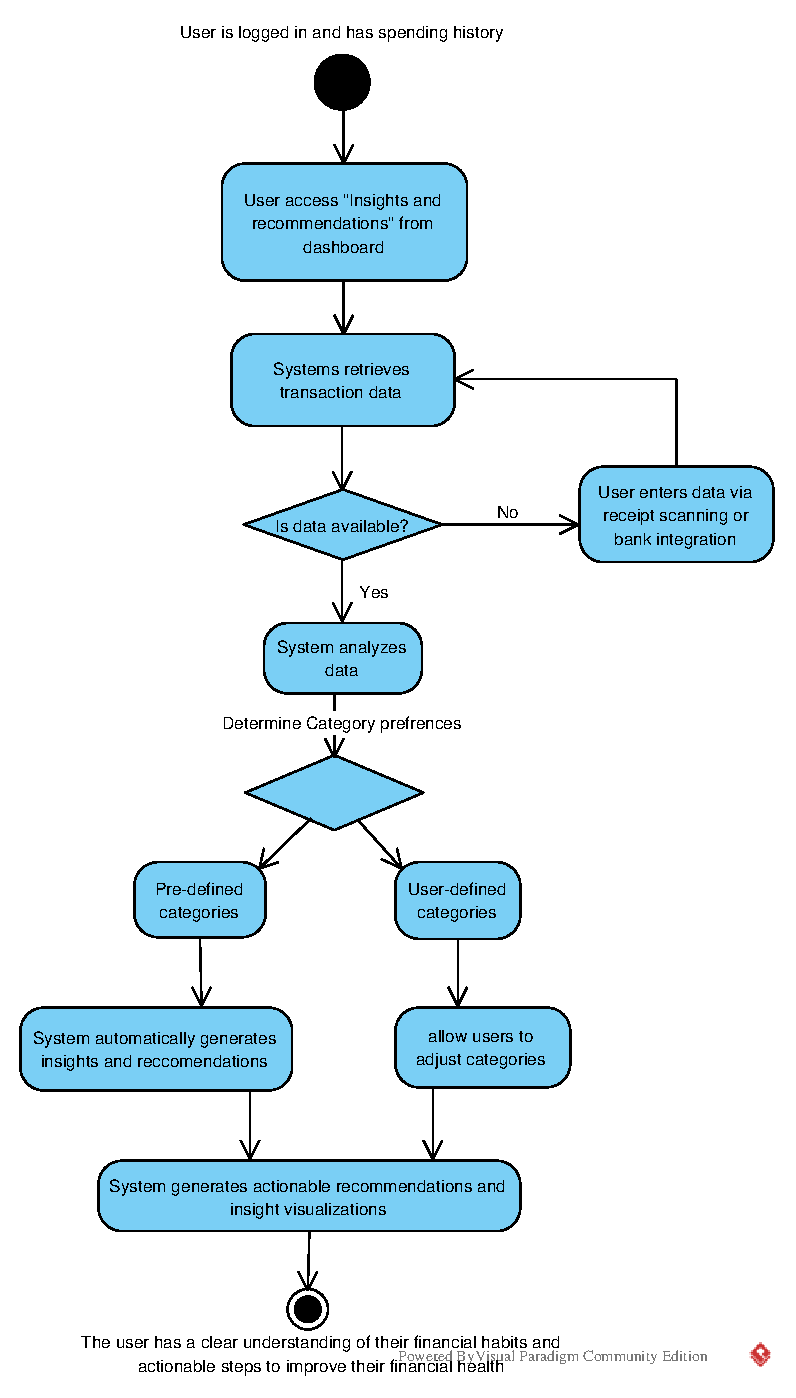
\includegraphics[width=0.5\linewidth]{eps/PFPActivityDiagramUC2.png.eps}
    \caption{Activity Diagram for Insights and Reccomendations}
    \label{fig:enter-label}
\end{figure}

\newpage

\subsection*{Use Case: Receipt Scanning}
\begin{useCase}[\UseCaseName{useCaseReceiptScanning}]
\UseCaseLabel{useCaseReceiptScanning} 
\end{useCase}

\subsubsection*{1. Name}
Receipt Scanning

\subsubsection*{2. Brief Description}
This use case allows the user to scan receipts using their mobile device camera or upload images of receipts. The system extracts transaction details such as total amount, date, and itemized purchases, categorizes the expenses, and updates the user's financial records automatically.

\subsubsection*{3. Actors}
\begin{itemize}
    \item \textbf{Primary Actor:} User
    \item \textbf{Supporting Actor:} AI Model (for receipt data extraction)
\end{itemize}

\subsubsection*{4. Basic Flow }
\begin{enumerate}
    \item The user accesses the "Receipt Scanning" feature from the application dashboard.
    \item The user takes a photo of a receipt or uploads an image from the device gallery.
    \item The system uses AI to process the image and extract data such as the date, total amount, and itemized details.
    \item The system categorizes the transaction into predefined or user-defined expense categories.
    \item The user reviews the extracted details and confirms them.
    \item The system saves the transaction data into the user's financial records.
\end{enumerate}

\subsubsection*{5. Alternate Flows (Rainy Day Scenarios)}
\begin{enumerate}[label=5.\arabic*]
    \item \textbf{Receipt unreadable due to poor image quality:}
    \begin{itemize}
        \item The system notifies the user and suggests rescanning the receipt or manually entering the details.
    \end{itemize}
    \item \textbf{User wishes to customize categories:}
    \begin{itemize}
        \item The system enables the user to define custom categories and reprocess the receipt for accurate categorization.
    \end{itemize}
\end{enumerate}

\subsubsection*{6. Exceptions}
\begin{enumerate}[label=6.\arabic*]
    \item \textbf{Receipt data extraction fails:}
    \begin{itemize}
        \item The system displays an error message and provides an option for manual data entry.
    \end{itemize}
    \item \textbf{Receipt upload fails due to connectivity issues:}
    \begin{itemize}
        \item The system notifies the user and suggests retrying once connectivity is restored.
    \end{itemize}
\end{enumerate}

\subsubsection*{7. Pre-Conditions}
\begin{itemize}
    \item The user must have the app installed on a device with a functioning camera or image upload capability.
    \item The user must be logged into the application.
\end{itemize}

\subsubsection*{8. Post-Conditions}
\begin{itemize}
    \item The receipt data is successfully extracted and categorized into the user's financial records.
    \item The user can view the updated records with categorized transactions.
\end{itemize}

\subsubsection*{9. Special Requirements}
\begin{itemize}
    \item The system should support multiple receipt formats and currencies.
    \item Ensure data privacy and encryption for receipt images and extracted data.
    \item The system must handle high volumes of receipt data efficiently.
    \item Provide transparency and minimize manual data entry for the user.
\end{itemize}

\subsubsection*{10. Engagement Considerations}
\begin{itemize}
    \item Provide a user-friendly interface for scanning or uploading receipts with minimal steps.
    \item Support for visually appealing confirmation screens (e.g., previews of extracted data).
    \item Offer light and dark modes for better accessibility.
\end{itemize}

\newpage

\begin{figure}[!h]
    \centering
    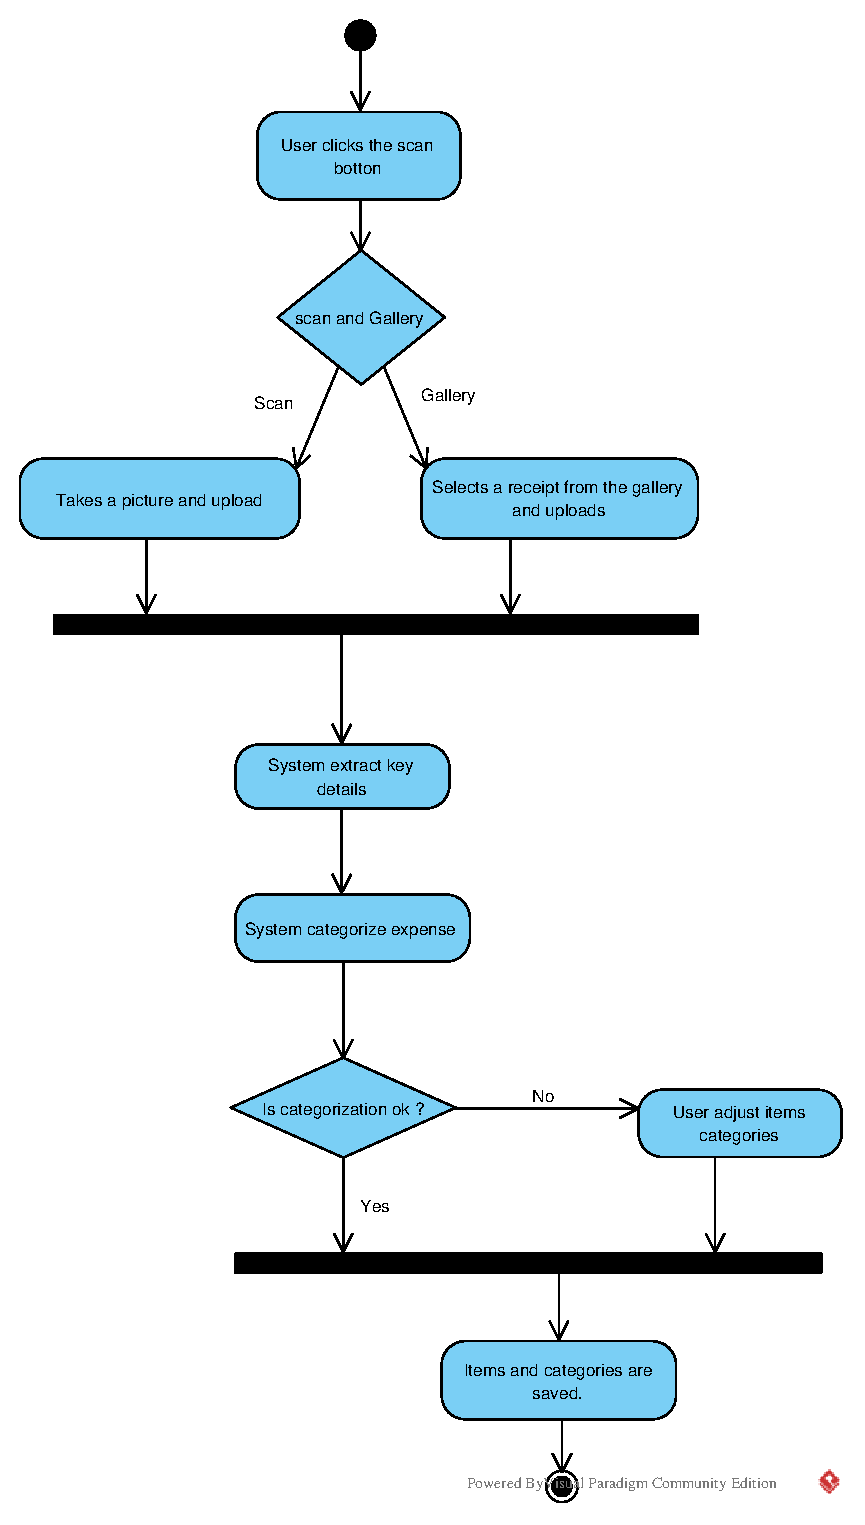
\includegraphics[width=0.5\linewidth]{eps/Receipt-Scanning.eps}
    \caption{Activity Diagram for Receipt Scanning}
    \label{fig:receiptScanning}
\end{figure}
\newpage


\subsection*{Use Case: Integrate Bank Account Transactions}
\begin{useCase}[\UseCaseName{useCaseBankAccountIntegration}]
\UseCaseLabel{useCaseBankAccountIntegration} 
\end{useCase}

\subsubsection*{1. Name}
Integrate Bank Account Transactions

\subsubsection*{2. Brief Description}
This use case allows the user to securely link their bank accounts to the application. The system fetches transaction details in real-time using webhook notifications and periodic pulls, categorizes them into predefined or user-defined categories, and updates the user's financial records automatically.

\subsubsection*{3. Actors}
\begin{itemize}
    \item \textbf{Primary Actor:} User
    \item \textbf{Supporting Actor:} Bank API
    \item \textbf{Supporting Actor:} Secure Data Processor (e.g., Plaid or similar service)
\end{itemize}

\subsubsection*{4. Basic Flow }
\begin{enumerate}
    \item The user accesses the "Bank Account Integration" feature from the application dashboard.
    \item The user selects a bank and is redirected to a secure authentication page provided by the Bank API.
    \item The user enters their bank credentials and grants permissions for the app to access transaction data.
    \item The system establishes a secure connection to the bank account.
    \item The system fetches existing transactions using a one-time pull request.
    \item The system sets up webhook notifications to receive real-time updates for new transactions.
    \item The system periodically pulls additional transaction data to ensure synchronization with the bank’s records.
    \item The system categorizes the transactions into predefined or user-defined categories.
    \item The user reviews and confirms the categorized transactions.
    \item The system saves the transactions into the user's financial records.
\end{enumerate}

\subsubsection*{5. Alternate Flows (Rainy Day Scenarios)}
\begin{enumerate}[label=5.\arabic*]
    \item \textbf{Webhook notification delivery fails:}
    \begin{itemize}
        \item The system detects the failure and switches to periodic pulls to fetch updates.
    \end{itemize}
    \item \textbf{Authentication fails:}
    \begin{itemize}
        \item The system notifies the user and provides an option to retry or contact support.
    \end{itemize}
    \item \textbf{Transaction data incomplete:}
    \begin{itemize}
        \item The system alerts the user and suggests manual review and categorization.
    \end{itemize}
\end{enumerate}

\subsubsection*{6. Exceptions}
\begin{enumerate}[label=6.\arabic*]
    \item \textbf{Bank API is unavailable:}
    \begin{itemize}
        \item The system displays an error message and provides an option to retry later.
    \end{itemize}
    \item \textbf{Webhook notifications stop unexpectedly:}
    \begin{itemize}
        \item The system sends a diagnostic report and switches to periodic pulls as a fallback mechanism.
    \end{itemize}
    \item \textbf{Connection timeout during transaction fetching:}
    \begin{itemize}
        \item The system retries fetching transactions up to three times before notifying the user.
    \end{itemize}
\end{enumerate}

\subsubsection*{7. Pre-Conditions}
\begin{itemize}
    \item The user must have the app installed and an active account.
    \item The user must have valid credentials for their bank account.
    \item The system must be configured to integrate with the selected bank’s API.
    \item The bank's API must support webhook notifications.
\end{itemize}

\subsubsection*{8. Post-Conditions}
\begin{itemize}
    \item The bank transactions are successfully fetched, categorized, and saved into the user's financial records.
    \item Real-time updates via webhooks are active and functioning correctly.
    \item Periodic pulls ensure the system is synchronized with the bank's records.
\end{itemize}

\subsubsection*{9. Special Requirements}
\begin{itemize}
    \item Ensure compliance with financial data protection laws (e.g., GDPR, CCPA).
    \item Use encryption for secure transmission and storage of bank account data.
    \item Support multiple banks and account types (savings, checking, credit, etc.).
    \item Provide clear error messages and recovery options for failed integrations.
    \item Webhooks must handle high availability and retry mechanisms for undelivered notifications.
\end{itemize}

\subsubsection*{10. Engagement Considerations}
\begin{itemize}
    \item Provide a seamless user experience for linking bank accounts with minimal steps.
    \item Offer an interactive walkthrough or help documentation for first-time users.
    \item Include visual indicators for integration progress, transaction updates, and webhook activity.
\    item Notify users immediately when webhooks detect significant events (e.g., new transactions).
\end{itemize}

\newpage

\subsection*{Use Case: Tax Filing}
\begin{useCase}[\UseCaseName{useCaseTaxFiling}]
\UseCaseLabel{useCaseTaxFiling} 
\end{useCase}

\subsubsection*{1. Name}
Tax Filing

\subsubsection*{2. Brief Description}
This use case enables users to automatically calculate, prepare, and file their taxes based on their financial data. The system aggregates income, expenses, and deductible items, applies relevant tax rules, and generates a ready-to-file tax report or submission.

\subsubsection*{3. Actors}
\begin{itemize}
    \item \textbf{Primary Actor:} User
    \item \textbf{Supporting Actor:} Tax Calculation Engine
    \item \textbf{Supporting Actor:} Tax Filing Service Provider (e.g., TurboTax API)
    \item \textbf{Supporting Actor:} Secure Data Processor
\end{itemize}

\subsubsection*{4. Basic Flow }
\begin{enumerate}
    \item The user accesses the "Tax Filing" feature from the application dashboard.
    \item The system aggregates the user’s financial data from linked accounts and categorized transactions.
    \item The system applies relevant tax laws based on the user's selected jurisdiction.
    \item A draft tax return is generated, showing income, deductions, and calculated tax liability or refunds.
    \item The user reviews the draft tax return for accuracy and completeness.
    \item The user selects an option to:
    \begin{itemize}
        \item Export the tax return for manual filing.
        \item File directly through an integrated e-filing service.
    \end{itemize}
    \item If e-filing is selected, the system submits the tax return electronically and provides a confirmation receipt.
\end{enumerate}

\subsubsection*{5. Alternate Flows (Rainy Day Scenarios)}
\begin{enumerate}[label=5.\arabic*]
    \item \textbf{Missing financial data:}
    \begin{itemize}
        \item The system detects missing information and prompts the user to input it manually.
    \end{itemize}
    \item \textbf{Tax filing error:}
    \begin{itemize}
        \item The system notifies the user of the error and suggests corrective actions.
    \end{itemize}
    \item \textbf{User disagrees with calculations:}
    \begin{itemize}
        \item The system allows the user to modify inputs and regenerates the tax return.
    \end{itemize}
\end{enumerate}

\subsubsection*{6. Exceptions}
\begin{enumerate}[label=6.\arabic*]
    \item \textbf{Tax rules outdated:}
    \begin{itemize}
        \item The system notifies the user of a temporary "Out of Service" status due to outdated tax rules.
        \item The system provides the following options:
        \begin{enumerate}[label=\alph*.]
            \item \textbf{Export Tax Data:} Allows the user to download relevant tax data (e.g., income, deductions, expenses) in a structured format (e.g., PDF, CSV) to assist with manual tax filing.
            \item \textbf{Notification Subscription:} Prompts the user to enable notifications to be informed when the system is updated and operational.
        \end{enumerate}
        \item The system reassures the user that tax rules are being updated by the system owner and will be restored soon.
    \end{itemize}
    \item \textbf{Submission failure:}
    \begin{itemize}
        \item The system retries the submission or advises the user to export and file manually.
    \end{itemize}
\end{enumerate}

\subsubsection*{7. Pre-Conditions}
\begin{itemize}
    \item The user must have synced all financial accounts with the app.
    \item The user must have selected their country and tax jurisdiction in the app settings.
    \item The system must be integrated with relevant tax filing APIs or systems.
\end{itemize}

\subsubsection*{8. Post-Conditions}
\begin{itemize}
    \item The tax return is successfully prepared and filed.
    \item A copy of the tax return and confirmation receipt is saved in the app for future reference.
\end{itemize}

\subsubsection*{9. Special Requirements}
\begin{itemize}
    \item The system must comply with tax regulations in supported jurisdictions.
    \item All financial data and tax-related information must be encrypted to ensure user privacy.
    \item Provide transparency in calculations with clear breakdowns of deductions and tax liabilities.
\end{itemize}

\subsubsection*{10. Engagement Considerations}
\begin{itemize}
    \item Include a step-by-step wizard to guide users through the tax filing process.
    \item Offer visual summaries, such as charts for income, deductions, and liabilities.
    \item Provide an FAQ section and tips to help users maximize deductions and credits.
\end{itemize}

\newpage


\subsection{Use Case 2: Receipt Scanning}

\subsubsection*{1. Name}
[Feature Name Placeholder]

\subsubsection*{2. Brief Description}
[Provide a short description of this use case.]

\subsubsection*{3. Actors}
[Identify the primary and supporting actors.]

\subsubsection*{4. Basic Flow (Sunny Day Scenario)}
\begin{enumerate}
    \item [Step 1...]
    \item [Step 2...]
\end{enumerate}

\subsubsection*{5. Alternate Flows (Rainy Day Scenarios)}
\begin{enumerate}[label=5.\arabic*]
    \item [Describe alternate flow...]
\end{enumerate}

\subsubsection*{6. Exceptions}
\begin{enumerate}[label=6.\arabic*]
    \item [Describe exception...]
\end{enumerate}

\subsubsection*{7. Pre-Conditions}

\subsection{Use Case 3: Bank Account Integration}

\subsection{Use Case 4: Budgeting Tools}

\subsection{Use Case 5: Tax Filing Assistance}
\newpage

\subsection{}
\begin{figure}[!h]
    \centering
    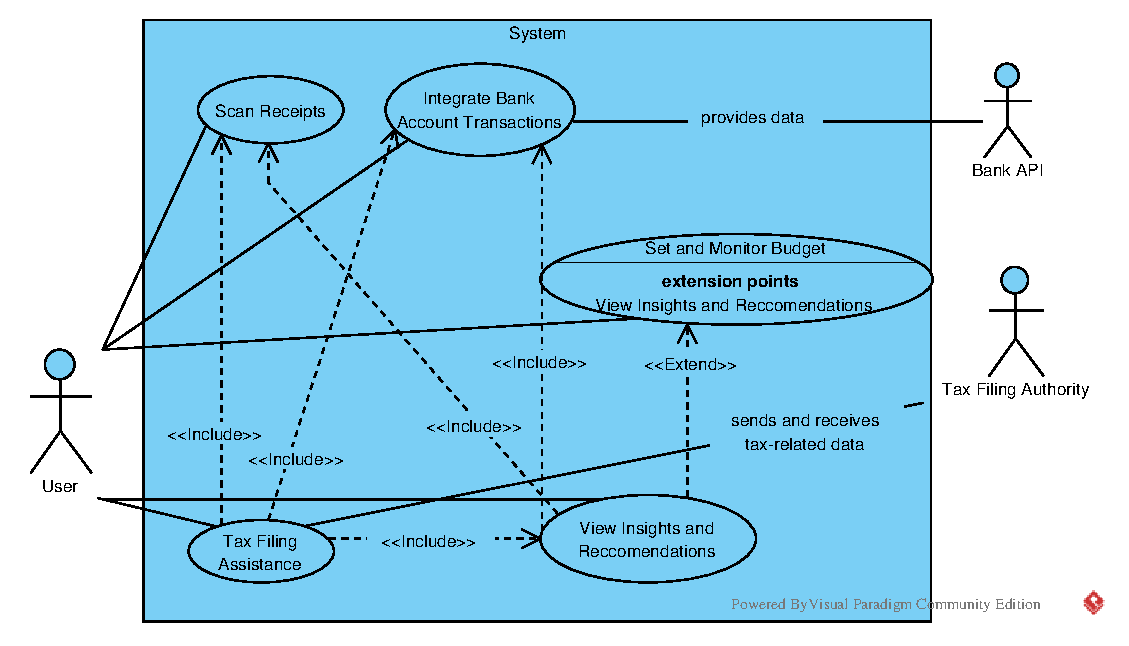
\includegraphics[width=0.7\linewidth]{eps/PFPUseCaseDiagram.eps}
    \caption{Personal Finance Tracker Use Case Diagram}
    \label{fig:PFP-usecase}
\end{figure}

\newpage
%-------------- Requirements -----------------------

\section{Requirements}

\begin{longtable}{|p{11cm}|p{3cm}|p{2cm}|}
\caption{Requirements Table}
\TableLabel{user_receipt_scanning_requirements}
\\
    \hline
    \textbf{User Requirement} & \textbf{Priority} & \textbf{Use Case} \\
    \hline

        \begin{reqkFunctional}[\RequirementName{reqkFunctional}{reqFInsightsDisplay}]
    \RequirementLabel{reqkFunctional}{reqFInsightsDisplay} 
    The app shall retrieve and display personalized financial insights and actionable recommendations based on the user's spending data and financial goals.
    \end{reqkFunctional} 
    &\vspace{0.5cm} \gls{must}\vspace{0.5cm} & \vspace{0.5cm} \UseCaseReference{useCaseViewingInsightsRecommendations} \vspace{0.5cm}  \\
    \hline

    \begin{reqkQuality}[\RequirementName{reqkQuality}{reqQInsightsAccuracy}]
    \RequirementLabel{reqkQuality}{reqQInsightsAccuracy} 
    The app shall ensure that 95\% of insights and recommendations provided to the user are accurate and relevant to their financial habits and goals.
    \end{reqkQuality} 
    &\vspace{0.5cm} \gls{must}\vspace{0.5cm} & \vspace{0.5cm} \UseCaseReference{useCaseViewingInsightsRecommendations} \vspace{0.5cm}  \\
    \hline

    \begin{reqkPerformance}[\RequirementName{reqkPerformance}{reqPInsightsSpeed}]
    \RequirementLabel{reqkPerformance}{reqPInsightsSpeed} 
    The app shall generate and display insights and recommendations within 3 seconds of accessing the feature, ensuring a smooth user experience.
    \end{reqkPerformance} 
    &\vspace{0.5cm} \gls{should}\vspace{0.5cm} & \vspace{0.5cm} \UseCaseReference{useCaseViewingInsightsRecommendations} \vspace{0.5cm}  \\
    \hline

    \begin{reqkSecurity}[\RequirementName{reqkSecurity}{reqSDataEncryption}]
    \RequirementLabel{reqkSecurity}{reqSDataEncryption} 
    The app shall encrypt all user data, including transaction details and insights, to protect user privacy and comply with data protection regulations.
    \end{reqkSecurity} 
    &\vspace{0.5cm} \gls{must}\vspace{0.5cm} & \vspace{0.5cm} \UseCaseReference{useCaseViewingInsightsRecommendations} \vspace{0.5cm}  \\
    \hline

    \begin{reqkBusiness}[\RequirementName{reqkBusiness}{reqBInsightsEngagement}]
    \RequirementLabel{reqkBusiness}{reqBInsightsEngagement} 
    The insights and recommendations feature shall increase user engagement by 25\% within the first six months of deployment through visually engaging and actionable insights.
    \end{reqkBusiness} 
    &\vspace{0.5cm} \gls{must}\vspace{0.5cm} & \vspace{0.5cm} \UseCaseReference{useCaseViewingInsightsRecommendations} \vspace{0.5cm}  \\
    \hline


%---------------------- Requirements 2 -----------------------

    \begin{reqkFunctional}[\RequirementName{reqkFunctional}{reqFReceiptScanning}]
    \RequirementLabel{reqkFunctional}{reqFReceiptScanning} 
    The system shall allow users to scan receipts using their mobile devices or upload receipt images to extract and categorize transaction details automatically.
    \end{reqkFunctional} 
    &\vspace{0.5cm} \gls{must}\vspace{0.5cm} & \vspace{0.5cm} \UseCaseReference{useCaseReceiptScanning} \vspace{0.5cm}  \\
    \hline

    \begin{reqkBusiness}[\RequirementName{reqkBusiness}{reqBReceiptScanningAdoption}]
    \RequirementLabel{reqkBusiness}{reqBReceiptScanningAdoption} 
    The receipt scanning feature shall improve user retention by 20\% within the first six months of deployment by reducing manual entry efforts and enhancing user convenience.
\end{reqkBusiness} 
&\vspace{0.5cm} \gls{must}\vspace{0.5cm} & \vspace{0.5cm} \UseCaseReference{useCaseReceiptScanning} \vspace{0.5cm}  \\
\hline


    \begin{reqkQuality}[\RequirementName{reqkQuality}{reqQReceiptAccuracy}]
    \RequirementLabel{reqkQuality}{reqQReceiptAccuracy} 
    The app’s receipt scanning feature shall achieve an accuracy rate of at least 95\% when extracting key details (e.g., total amount, date, and itemized purchases) from standard receipt formats.
    \end{reqkQuality} 
    &\vspace{0.5cm} \gls{must}\vspace{0.5cm} & \vspace{0.5cm} \UseCaseReference{useCaseReceiptScanning} \vspace{0.5cm}  \\
    \hline

    \begin{reqkPerformance}[\RequirementName{reqkPerformance}{reqPReceiptSpeed}]
    \RequirementLabel{reqkPerformance}{reqPReceiptSpeed} 
    The app shall process scanned receipts within 5 seconds to provide a seamless user experience.
    \end{reqkPerformance} 
    &\vspace{0.5cm} \gls{should}\vspace{0.5cm} & \vspace{0.5cm} \UseCaseReference{useCaseReceiptScanning} \vspace{0.5cm}  \\
    \hline

    \begin{reqkSecurity}[\RequirementName{reqkSecurity}{reqSReceiptDataSecurity}]
    \RequirementLabel{reqkSecurity}{reqSReceiptDataSecurity} 
    The app shall encrypt all receipt images and extracted data to ensure user privacy and comply with data protection regulations.
    \end{reqkSecurity} 
    &\vspace{0.5cm} \gls{must}\vspace{0.5cm} & \vspace{0.5cm} \UseCaseReference{useCaseReceiptScanning} \vspace{0.5cm}  \\
    \hline

%-------------- Requirements 3 --------------------------------------

\begin{reqkFunctional}[\RequirementName{reqkFunctional}{reqFBankIntegration}]
    \RequirementLabel{reqkFunctional}{reqFBankIntegration} 
    The system shall allow users to securely link their bank accounts and fetch transaction details automatically via API integrations.
\end{reqkFunctional} 
&\vspace{0.5cm} \gls{must}\vspace{0.5cm} & \vspace{0.5cm} \UseCaseReference{useCaseBankAccountIntegration} \vspace{0.5cm}  \\
\hline

\begin{reqkBusiness}[\RequirementName{reqkBusiness}{reqBBankIntegrationRetention}]
    \RequirementLabel{reqkBusiness}{reqBBankIntegrationRetention} 
    The bank account integration feature shall improve user retention by 30\% within the first six months of deployment by eliminating the need for manual transaction entry and providing real-time updates.
\end{reqkBusiness} 
&\vspace{0.5cm} \gls{must}\vspace{0.5cm} & \vspace{0.5cm} \UseCaseReference{useCaseBankAccountIntegration} \vspace{0.5cm}  \\
\hline

\begin{reqkQuality}[\RequirementName{reqkQuality}{reqQBankDataAccuracy}]
    \RequirementLabel{reqkQuality}{reqQBankDataAccuracy} 
    The app shall categorize fetched transactions with an accuracy rate of at least 95\%, aligning them with user-defined or predefined categories.
\end{reqkQuality} 
&\vspace{0.5cm} \gls{must}\vspace{0.5cm} & \vspace{0.5cm} \UseCaseReference{useCaseBankAccountIntegration} \vspace{0.5cm}  \\
\hline

\begin{reqkPerformance}[\RequirementName{reqkPerformance}{reqPBankIntegrationSpeed}]
    \RequirementLabel{reqkPerformance}{reqPBankIntegrationSpeed} 
    The app shall fetch and process bank transactions within 3 seconds per API request to ensure a seamless user experience.
\end{reqkPerformance} 
&\vspace{0.5cm} \gls{should}\vspace{0.5cm} & \vspace{0.5cm} \UseCaseReference{useCaseBankAccountIntegration} \vspace{0.5cm}  \\
\hline

\begin{reqkSecurity}[\RequirementName{reqkSecurity}{reqSBankDataSecurity}]
    \RequirementLabel{reqkSecurity}{reqSBankDataSecurity} 
    The app shall encrypt all bank account data, including transaction details, to ensure user privacy and comply with financial data protection regulations (e.g., GDPR, CCPA).
\end{reqkSecurity} 
&\vspace{0.5cm} \gls{must}\vspace{0.5cm} & \vspace{0.5cm} \UseCaseReference{useCaseBankAccountIntegration} \vspace{0.5cm}  \\
\hline

\begin{reqkFunctional}[\RequirementName{reqkFunctional}{reqFWebhookSupport}]
    \RequirementLabel{reqkFunctional}{reqFWebhookSupport} 
    The system shall support webhook notifications from the bank’s API to provide real-time transaction updates.
\end{reqkFunctional} 
&\vspace{0.5cm} \gls{must}\vspace{0.5cm} & \vspace{0.5cm} \UseCaseReference{useCaseBankAccountIntegration} \vspace{0.5cm}  \\
\hline

\begin{reqkPerformance}[\RequirementName{reqkPerformance}{reqPWebhookResponse}]
    \RequirementLabel{reqkPerformance}{reqPWebhookResponse} 
    The system shall process webhook notifications and update user financial records within 2 seconds of receiving the notification.
\end{reqkPerformance} 
&\vspace{0.5cm} \gls{should}\vspace{0.5cm} & \vspace{0.5cm} \UseCaseReference{useCaseBankAccountIntegration} \vspace{0.5cm}  \\
\hline

\begin{reqkBusiness}[\RequirementName{reqkBusiness}{reqBWebhookAdoption}]
    \RequirementLabel{reqkBusiness}{reqBWebhookAdoption} 
    The webhook integration feature shall reduce the average user session time for transaction updates by 50\%, improving user satisfaction with real-time updates.
\end{reqkBusiness} 
&\vspace{0.5cm} \gls{must}\vspace{0.5cm} & \vspace{0.5cm} \UseCaseReference{useCaseBankAccountIntegration} \vspace{0.5cm}  \\
\hline

\begin{reqkFunctional}[\RequirementName{reqkFunctional}{reqFTaxDataAggregation}]
    \RequirementLabel{reqkFunctional}{reqFTaxDataAggregation} 
    The system shall aggregate the user’s financial data from linked accounts, categorized transactions, and manual inputs to prepare a tax return.
\end{reqkFunctional} 
&\vspace{0.5cm} \gls{must}\vspace{0.5cm} & \vspace{0.5cm} \UseCaseReference{useCaseTaxFiling} \vspace{0.5cm}  \\
\hline

\begin{reqkFunctional}[\RequirementName{reqkFunctional}{reqFTaxRulesApplication}]
    \RequirementLabel{reqkFunctional}{reqFTaxRulesApplication} 
    The system shall apply tax rules based on the user’s selected jurisdiction to calculate income, deductions, and tax liability or refunds.
\end{reqkFunctional} 
&\vspace{0.5cm} \gls{must}\vspace{0.5cm} & \vspace{0.5cm} \UseCaseReference{useCaseTaxFiling} \vspace{0.5cm}  \\
\hline

\begin{reqkFunctional}[\RequirementName{reqkFunctional}{reqFTaxFilingOptions}]
    \RequirementLabel{reqkFunctional}{reqFTaxFilingOptions} 
    The system shall allow users to either export the tax return for manual filing or file it directly through an integrated e-filing service.
\end{reqkFunctional} 
&\vspace{0.5cm} \gls{must}\vspace{0.5cm} & \vspace{0.5cm} \UseCaseReference{useCaseTaxFiling} \vspace{0.5cm}  \\
\hline

\begin{reqkBusiness}[\RequirementName{reqkBusiness}{reqBTaxFilingConvenience}]
    \RequirementLabel{reqkBusiness}{reqBTaxFilingConvenience} 
    The tax filing feature shall increase user satisfaction by 25\% within the first six months of deployment by automating the preparation and filing process.
\end{reqkBusiness} 
&\vspace{0.5cm} \gls{must}\vspace{0.5cm} & \vspace{0.5cm} \UseCaseReference{useCaseTaxFiling} \vspace{0.5cm}  \\
\hline

\begin{reqkQuality}[\RequirementName{reqkQuality}{reqQTaxCalculationAccuracy}]
    \RequirementLabel{reqkQuality}{reqQTaxCalculationAccuracy} 
    The system shall achieve an accuracy rate of at least 98\% in applying tax rules and calculating liabilities or refunds.
\end{reqkQuality} 
&\vspace{0.5cm} \gls{must}\vspace{0.5cm} & \vspace{0.5cm} \UseCaseReference{useCaseTaxFiling} \vspace{0.5cm}  \\
\hline

\begin{reqkPerformance}[\RequirementName{reqkPerformance}{reqPTaxProcessingSpeed}]
    \RequirementLabel{reqkPerformance}{reqPTaxProcessingSpeed} 
    The system shall generate a complete tax return within 10 seconds after gathering all required inputs.
\end{reqkPerformance} 
&\vspace{0.5cm} \gls{should}\vspace{0.5cm} & \vspace{0.5cm} \UseCaseReference{useCaseTaxFiling} \vspace{0.5cm}  \\
\hline

\begin{reqkSecurity}[\RequirementName{reqkSecurity}{reqSTaxDataSecurity}]
    \RequirementLabel{reqkSecurity}{reqSTaxDataSecurity} 
    The system shall encrypt all financial and tax-related data to ensure user privacy and compliance with data protection regulations (e.g., GDPR, CCPA).
\end{reqkSecurity} 
&\vspace{0.5cm} \gls{must}\vspace{0.5cm} & \vspace{0.5cm} \UseCaseReference{useCaseTaxFiling} \vspace{0.5cm}  \\
\hline

\begin{reqkFunctional}[\RequirementName{reqkFunctional}{reqFTaxOutdatedRulesHandling}]
    \RequirementLabel{reqkFunctional}{reqFTaxOutdatedRulesHandling} 
    The system shall notify users of a temporary "Out of Service" status when tax rules are outdated, and provide options to export tax data for manual filing and enable notifications for updates.
\end{reqkFunctional} 
&\vspace{0.5cm} \gls{must}\vspace{0.5cm} & \vspace{0.5cm} \UseCaseReference{useCaseTaxFiling} \vspace{0.5cm}  \\
\hline

\begin{reqkBusiness}[\RequirementName{reqkBusiness}{reqBTaxManualAssistance}]
    \RequirementLabel{reqkBusiness}{reqBTaxManualAssistance} 
    The system shall reduce the time users spend on manual tax filing by 40\% by providing well-organized tax data exports during service disruptions.
\end{reqkBusiness} 
&\vspace{0.5cm} \gls{should}\vspace{0.5cm} & \vspace{0.5cm} \UseCaseReference{useCaseTaxFiling} \vspace{0.5cm}  \\
\hline


\end{longtable}

%---------------------------------------
\newpage
\section{Traceability Matrix}
% Include both tables to trace Use Case to Requirements and Requirements to Use Cases 

\subsection{Use Cases-to-Requirements Table:}

\begin{longtable}{|m{8cm}|m{6cm}|}
\caption{Use Case and Requirement Coverage Table \label{table:use-case-requirements}} \\

    \hline
    \textbf{Use Case ID and Description} & \textbf{Linked Requirements} \\
    \hline
    \endfirsthead

    \hline
    \textbf{Use Case ID and Description} & \textbf{Linked Requirements} \\
    \hline
    \endhead

    % Use Case: Viewing Insights and Recommendations
    \UseCaseReference{useCaseViewingInsightsRecommendations}: Viewing Insights and Recommendations - Allows users to view personalized financial insights and actionable recommendations based on their spending habits and financial goals.
    & \vspace{0.2cm}
      \begin{itemize}[leftmargin=*]
        \item \RequirementReference{reqkFunctional}{reqFInsightsDisplay}
        \item \RequirementReference{reqkQuality}{reqQInsightsAccuracy}
        \item \RequirementReference{reqkPerformance}{reqPInsightsSpeed}
        \item \RequirementReference{reqkBusiness}{reqBInsightsEngagement}
      \end{itemize} \\
    \hline

    % Use Case: Receipt Scanning and Expense Analysis
    \UseCaseReference{useCaseReceiptScanning}: Receipt Scanning and Expense Analysis - Enables users to scan or upload receipts, extract transaction details, and categorize expenses automatically.
    & \vspace{0.2cm}
      \begin{itemize}[leftmargin=*]
        \item \RequirementReference{reqkFunctional}{reqFReceiptScanning}
        \item \RequirementReference{reqkQuality}{reqQReceiptAccuracy}
        \item \RequirementReference{reqkPerformance}{reqPReceiptSpeed}
        \item \RequirementReference{reqkSecurity}{reqSDataEncryption}
      \end{itemize} \\
    \hline

    % Use Case: Integrate Bank Account Transactions
    \UseCaseReference{useCaseBankAccountIntegration}: Integrate Bank Account Transactions - Allows users to securely link their bank accounts, fetch transactions automatically, and categorize them into expense categories using webhooks and periodic pulls.
    & \vspace{0.2cm}
      \begin{itemize}[leftmargin=*]
        \item \RequirementReference{reqkFunctional}{reqFBankIntegration}
        \item \RequirementReference{reqkQuality}{reqQBankDataAccuracy}
        \item \RequirementReference{reqkPerformance}{reqPBankIntegrationSpeed}
        \item \RequirementReference{reqkSecurity}{reqSBankDataSecurity}
        \item \RequirementReference{reqkFunctional}{reqFWebhookSupport}
      \end{itemize} \\
    \hline

    % Use Case: Tax Filing
    \UseCaseReference{useCaseTaxFiling}: Tax Filing - Enables users to calculate, prepare, and file taxes automatically based on their financial data, applying jurisdiction-specific rules and generating ready-to-file tax returns.
    & \vspace{0.2cm}
      \begin{itemize}[leftmargin=*]
        \item \RequirementReference{reqkFunctional}{reqFTaxDataAggregation}
        \item \RequirementReference{reqkFunctional}{reqFTaxRulesApplication}
        \item \RequirementReference{reqkFunctional}{reqFTaxFilingOptions}
        \item \RequirementReference{reqkQuality}{reqQTaxCalculationAccuracy}
        \item \RequirementReference{reqkPerformance}{reqPTaxProcessingSpeed}
        \item \RequirementReference{reqkSecurity}{reqSTaxDataSecurity}
        \item \RequirementReference{reqkFunctional}{reqFTaxOutdatedRulesHandling}
      \end{itemize} \\
    \hline

\end{longtable}



\section{Requirement Elicitation Process}

\subsection{Domain Analysis}
\subsubsection{Purpose}
The purpose of domain analysis was to identify essential functionalities and missing features by analyzing existing systems and understanding their strengths and gaps.

\subsubsection{Methodology}
\begin{itemize}
    \item Evaluated competitor applications such as \textit{Mint} and \textit{YNAB}.
    \item Identified features that differentiate the Personal Finance Tracker, such as receipt scanning and automated tax calculations.
    \item Analyzed gaps in existing tools to recommend additional functionalities for an improved user experience.
\end{itemize}

\subsubsection{Results}
Key findings from domain analysis include:
\begin{itemize}
    \item Real-time spending alerts were identified as critical for enhancing user awareness.
    \item Integration with investment platforms and bank accounts to streamline data collection.
    \item Customizable reporting tools for better insights into spending patterns.
\end{itemize}

\subsection{Interviews}
\subsubsection{Purpose}
The purpose of conducting interviews was to validate assumptions about user pain points, gather insights on priorities, and understand how users interact with financial management tools.

\subsubsection{Interview Participants}
We interviewed a diverse group of users who could represent the primary user classes for the Personal Finance Tracker:

\begin{itemize}
    \item \textbf{Padma Setty} - Family Member; Working professional with regular expenses.
    \item \textbf{Paul Baccaglini} - Classmate; University student managing limited income.
    \item \textbf{Isibeal Snowhill} - Roommate; University Student managing financial aid and low income. 
    \item \textbf{} - 
    \item \textbf{} - 
\end{itemize}

\subsubsection{Methodology}
The interviews were conducted in a semi-structured format using the following questions:

\begin{enumerate}
    \item How do you currently manage your finances? (e.g., spreadsheets, apps, advisors)
    \item What challenges do you face with your current method of managing finances?
    \item How important are budgeting tools, spending alerts, and financial insights to your goals?
    \item Would you use a feature that scans receipts and automatically categorizes expenses? Why or why not?
    \item What would encourage you to integrate your bank account with a financial tracking app?
    \item How important is security and privacy when sharing your financial data with an app?
    \item Do you currently file taxes manually or use software? What challenges do you face with tax preparation?
    \item Would you benefit from receiving personalized insights and recommendations about your spending habits?
    \item How frequently would you use a personal finance tracker (e.g., daily, weekly, monthly)?
    \item Rank the importance of the following features for you: 
    \begin{itemize}
        \item Budgeting tools and spending alerts.
        \item Receipt scanning and automated expense categorization.
        \item Insights and recommendations for saving and spending.
        \item Automated tax filing assistance.
    \end{itemize}
\end{enumerate}

\subsubsection{Results}
Key findings from the interviews are as follows:
\begin{itemize}
    \item \textbf{Working Individuals:}
    \begin{itemize}
        \item Budgeting tools and spending alerts were ranked as the most important features, followed by receipt scanning and financial insights.
        \item Automated tax filing assistance was beneficial but seen as secondary to daily financial management.
        \item Security measures, such as two-factor authentication and encryption, were considered essential for trust.
    \end{itemize}
    \item \textbf{Students:}
    \begin{itemize}
        \item Budgeting tools and expense categorization were highlighted as the most useful features.
        \item Real-time alerts for overspending were seen as valuable for controlling expenses.
        \item Simple and clear visualizations (e.g., spending graphs) were preferred for better financial awareness.
    \end{itemize}
\end{itemize}

\subsection{Scenarios}
\subsubsection{Purpose}
The purpose of scenario development was to simulate practical user interactions with the system to validate the relevance of features and ensure alignment with real-world needs.

\subsubsection{Methodology}
\begin{itemize}
    \item Developed scenarios based on use cases to illustrate interactions such as:
        \begin{itemize}
            \item A working individual scanning receipts and generating spending insights.
            \item A student receiving real-time alerts when approaching their food budget limit.
        \end{itemize}
    \item Highlighted pain points such as manual effort in financial management and the need for actionable insights.
    \item Evaluated system responses to ensure features address user priorities effectively.
\end{itemize}

\subsubsection{Results}
Key findings from scenarios include:
\begin{itemize}
    \item Scenarios validated alignment of the proposed features with user needs.
    \item Emphasis on automation, simplicity, and actionable feedback was critical for user satisfaction.
    \item Supported the prioritization of core functionalities, such as:
        \begin{itemize}
            \item Budgeting tools and spending alerts.
            \item Insights and recommendations for improved financial decisions.
            \item Automated tax filing assistance.
        \end{itemize}
\end{itemize}



%-------------------------------------------------------------



%-------------------------------- Requirements Analysis-------

\newpage
\section{Requirements Analysis}

\subsection{Requirements Analysis Methodology and Tool}
The requirements analysis conducted for the Personal Finance Tracker app uses a structured framework. This methodology combines the following approaches:
\begin{itemize}
    \item \textbf{Functional and Non-Functional Analysis:} Identify core functionalities and assess non-functional attributes like quality, performance, and security.
    \item \textbf{Risk-Based Analysis:} Highlight potential challenges and risks, including dependencies and external integration issues.
    \item \textbf{Dependency Analysis:} Evaluate relationships between system components, external APIs, and AI/ML systems.
    \item \textbf{Prioritization Analysis:} Classify requirements into high and medium priorities based on their criticality.
    \item \textbf{Alignment with Stakeholder Goals:} Align requirements with user and business needs to ensure system value delivery.
    \item \textbf{Feasibility and Scalability Analysis:} Assess the technical feasibility and scalability for future growth.
    \item \textbf{Standards-Based Analysis:} Ensure compliance with industry standards like GDPR and CCPA.
    \item \textbf{Key Metrics Definition:} Define measurable goals to ensure each requirement is verifiable and achievable.
\end{itemize}
This approach ensures that the analysis is comprehensive, actionable, and aligned with best practices in software engineering.

\subsection{Requirements Analysis - Viewing Insights and Recommendations}
\begin{itemize}
    \item \textbf{Functional Requirements:}
    \begin{itemize}
        \item The app must retrieve and display personalized financial insights and recommendations based on user data.
        \item \textbf{Analysis:} This aligns directly with the core functionality and addresses user needs for personalization. It depends on reliable integration with bank APIs and data sources.
        \item \textbf{Risk/Challenge:} Data inconsistency from external APIs may impact insights quality.
    \end{itemize}
    
    \item \textbf{Quality Requirements:}
    \begin{itemize}
        \item The app shall ensure that 95\% of insights are accurate and relevant.
        \item \textbf{Analysis:} Accuracy builds user trust and satisfaction, requiring robust algorithms.
        \item \textbf{Risk/Challenge:} Diverse user data formats and behaviors might reduce relevance.
    \end{itemize}
    
    \item \textbf{Performance Requirements:}
    \begin{itemize}
        \item Insights must be generated within 3 seconds for seamless user experience.
        \item \textbf{Analysis:} This ensures responsiveness and enhances user satisfaction.
        \item \textbf{Risk/Challenge:} Handling large datasets during peak loads may cause delays.
    \end{itemize}
    
    \item \textbf{Security Requirements:}
    \begin{itemize}
        \item Encrypt user data to comply with GDPR and protect user privacy.
        \item \textbf{Analysis:} Security builds user trust and ensures compliance with regulations.
        \item \textbf{Risk/Challenge:} Robust encryption may impact performance slightly.
    \end{itemize}
    
    \item \textbf{Business Requirements:}
    \begin{itemize}
        \item The feature should increase user engagement by 25\% within six months.
        \item \textbf{Analysis:} Visually engaging insights and actionable recommendations support this.
        \item \textbf{Risk/Challenge:} Insights must address meaningful financial pain points.
    \end{itemize}
\end{itemize}

\subsection{Requirements Analysis - Receipt Scanning and Expense Analysis}
\begin{itemize}
    \item \textbf{Functional Requirements:}
    \begin{itemize}
        \item The app shall allow users to scan or upload receipts to extract and categorize expense details automatically.
        \item \textbf{Analysis:} Automating expense categorization saves user time and improves accuracy. It relies on advanced AI/ML models.
        \item \textbf{Risk/Challenge:} Poor image quality or non-standard receipt formats may reduce reliability.
    \end{itemize}
    
    \item \textbf{Quality Requirements:}
    \begin{itemize}
        \item Receipt scanning accuracy must achieve 95\% for standard receipt formats.
        \item \textbf{Analysis:} High accuracy ensures reliable data extraction and user satisfaction.
        \item \textbf{Risk/Challenge:} Non-standard or handwritten receipts might reduce extraction accuracy.
    \end{itemize}
    
    \item \textbf{Performance Requirements:}
    \begin{itemize}
        \item Receipts must be processed within 5 seconds.
        \item \textbf{Analysis:} Fast processing ensures a smooth and efficient user experience.
        \item \textbf{Risk/Challenge:} Complex or long receipts may require additional processing time.
    \end{itemize}
    
    \item \textbf{Security Requirements:}
    \begin{itemize}
        \item Encrypt all receipt images and extracted data to ensure privacy and compliance with regulations.
        \item \textbf{Analysis:} Encryption ensures user data remains secure and meets compliance standards.
        \item \textbf{Risk/Challenge:} Implementing secure data handling without sacrificing performance requires optimization.
    \end{itemize}
    
    \item \textbf{Business Requirements:}
    \begin{itemize}
        \item Automating expense tracking should increase user retention by 20\% within the first six months.
        \item \textbf{Analysis:} Automation reduces manual effort and enhances app usability.
        \item \textbf{Risk/Challenge:} Poor feature usability may lead to user churn.
    \end{itemize}
\end{itemize}


%-------------------------------------------------------------
\section{Requirements Management}
Talk about using JIRA + issue tracking 
Include screenshots and Links 